% Einleitung.tex

% Definiere Variablen
% \newcommand{\Messziel}{Messziel}

\newcommand{\Motivation}{
    % Hier Motivation einfügen
    Ziel dieser Arbeit ist es, die Grenzen von Threads und Parallelisierung aufzuzeigen. Dabei soll insbesondere untersucht werden, wie groß der Overhead durch Threads ist und welchen Performanceunterschied es macht, bereits initialisierte Workerthreads zu verwenden, im Vergleich zur Erstellung neuer Threads.
    Da sich für diese Untersuchungen ein geeigneter, leicht verständlicher und programmierbarer Anwendungsfall anbietet, habe ich mich für Sortieralgorithmen entschieden, die sich zudem sehr gut parallelisieren lassen.
}

\newcommand{\ZielsetzungUndForschungsfrage}{
    % Hier Zielsetzung und Forschungsfrage einfügen
    Ziel dieser Bachelorarbeit ist die systematische Analyse der Laufzeitentwicklung paralleler Sortierverfahren. Dabei soll untersucht werden, wie sich parallele Implementierungen von Quicksort und Mergesort im Vergleich zu ihren sequentiellen Varianten verhalten.
    Im Fokus stehen insbesondere folgende Punkte:
    \begin{itemize}
        \item der Einfluss verschiedener Threadingstrategien auf die Laufzeit,
        \item die Frage, ab welcher Eingangsgröße und bei welcher Anzahl von Threads ein messbarer Geschwindigkeitsvorteil entsteht,
        \item sowie die Identifikation von Thread-Management-Techniken, die für Sortieralgorithmen die besten Laufzeiten erzielen.
    \end{itemize}
    Aus diesen Aspekten ergibt sich die zentrale Forschungsfrage dieser Arbeit:
    \newline
    \textbf{Unter welchen Bedingungen liefern parallele Sortieralgorithmen anhand von Quicksort und Mergesort einen signifikanten Laufzeitvorteil gegenüber der sequentiellen Ausführung, und welche Threadingstrategien führen dabei zur besten Laufzeit?}
}

\newcommand{\InkrementArrayDiagrammA}{%
    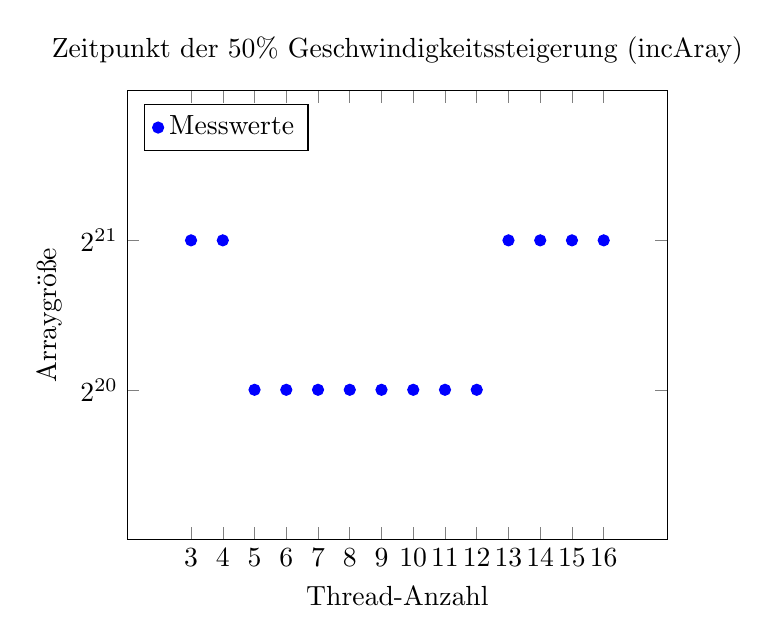
\begin{tikzpicture}
        \begin{axis}[
                xlabel={Thread-Anzahl},
                ylabel={Arraygröße},
                title={Zeitpunkt der 50\% Geschwindigkeitssteigerung (incAray)},
                xmin=1, xmax=18,
                ymin=2^19, ymax=2^22,
                grid style=dashed,
                legend pos=north west,
                ymode=log,
                log basis y=2,
                xtick={3,...,16},               % jeden Integer von 2 bis 17
                ytick={2^20,2^21},      % gewünschte y-Werte
                % yticklabels={\ensuremath{2^{19}},\ensuremath{2^{20}},\ensuremath{2^{21}},\ensuremath{2^{22}},\ensuremath{2^{23}}} % Beschriftung
            ]
            \addplot[only marks, blue, mark=*] coordinates {
                    (1,2)
                    (3,2097152)
                    (4,2097152)
                    (5,1048576)
                    (6,1048576)
                    (7,1048576)
                    (8,1048576)
                    (9,1048576)
                    (10,1048576)
                    (11,1048576)
                    (12,1048576)
                    (13,2097152)
                    (14,2097152)
                    (15,2097152)
                    (16,2097152)
                };
            \addlegendentry{Messwerte}
        \end{axis}
    \end{tikzpicture}%
}

\newcommand{\InkrementArrayDiagrammB}{%
    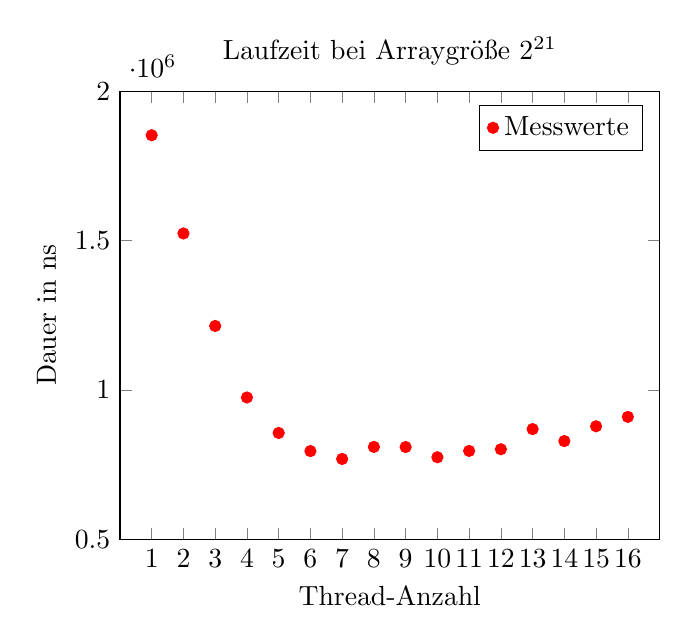
\begin{tikzpicture}
        \begin{axis}[
                xlabel={Thread-Anzahl},
                ylabel={Dauer in ns},
                title={Laufzeit bei Arraygröße $2^{21}$},
                xmin=0, xmax=17,
                ymin=0.5*10^6, ymax=2*10^6,
                grid style=dashed,
                legend pos=north east,
                xtick={1,...,16},
                % ymode=log,
            ]
            \addplot[only marks, red, mark=*] coordinates {
                    (1,1852600)
                    (2,1524000)
                    (3,1214400)
                    (4,975200)
                    (5,856500)
                    (6,795800)
                    (7,769500)
                    (8,809800)
                    (9,809400)
                    (10,775200)
                    (11,796400)
                    (12,802000)
                    (13,869400)
                    (14,829300)
                    (15,878800)
                    (16,910300)
                };
            \addlegendentry{Messwerte}
        \end{axis}
    \end{tikzpicture}%
}

\newcommand{\InkrementArrayDiagrammC}{%
    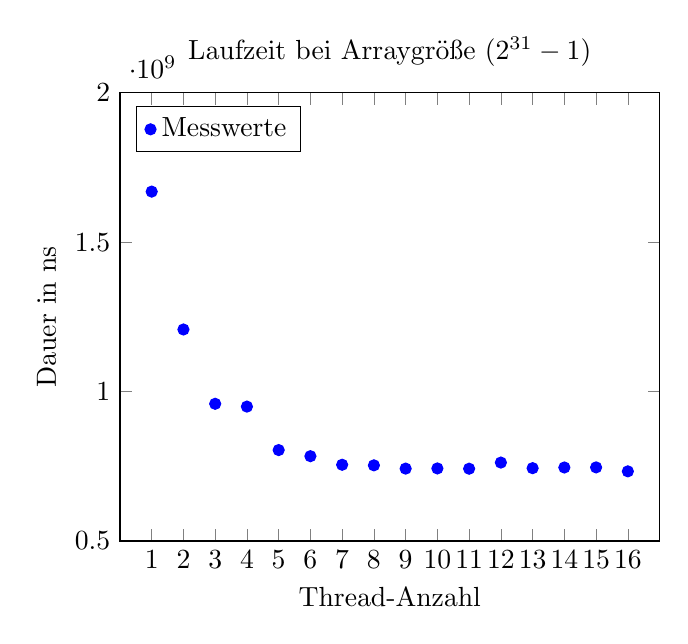
\begin{tikzpicture}
        \begin{axis}[
                xlabel={Thread-Anzahl},
                ylabel={Dauer in ns},
                title={Laufzeit bei Arraygröße ($2^{31}-1$)},
                xmin=0, xmax=17,
                ymin=0.5*10^9, ymax=0.2*10^10,
                grid style=dashed,
                legend pos=north west,
                xtick={1,...,16},
            ]
            \addplot[only marks, blue, mark=*] coordinates {
                    (1,1669092400)
                    (2,1207814700)
                    (3,959192500)
                    (4,949815500)
                    (5,804376400)
                    (6,783903900)
                    (7,755204600)
                    (8,753302500)
                    (9,742325400)
                    (10,742938600)
                    (11,741977000)
                    (12,762527700)
                    (13,743848100)
                    (14,746071200)
                    (15,746385900)
                    (16,733162900)
                };
            \addlegendentry{Messwerte}
        \end{axis}
    \end{tikzpicture}%
}

\newcommand{\InkrementArray}{
    % Inkrement-Array
    \InkrementArrayDiagrammA
    \newline
    \InkrementArrayDiagrammB
    \newline
    \InkrementArrayDiagrammC
}